\section{Controlled Analyses (C2)}

Each of the seven analyses follows the same four-part structure --- the
question, the design, the control that bites, and the finding with its bound ---
and in four of the seven the control that bites took down a claim of our own.
One caveat belongs before the first of them: the seven are not seven independent
studies. The displacement analysis in \S\ref{sec:e1v3} and the exploratory
cross-layer association (Supplementary Note S2) share a panel, an estimator and
the same November 2019 event, so the latter is in substance an audit of the
former that found the pre-trend the earlier design had missed. The number of
independent events behind this corpus is therefore smaller than seven.
Table~\ref{tab:analyses} gives the whole corpus at a glance; full controls and
every rejected estimator are in Supplementary Note S2.

\begin{table}[t]
\caption{The seven controlled analyses: the quantity that survived each one, the
layer it belongs to, the control that bit, and what that control rejected. Four
of the seven controls took down a claim of our own.\label{tab:analyses}}
\scriptsize
\setlength{\tabcolsep}{3pt}
\begin{tabular}{@{}L{1.75cm}L{1.55cm}L{4.35cm}L{3.35cm}L{5.0cm}@{}}
\toprule
\textbf{Analysis} & \textbf{Layer} & \textbf{Headline quantity} & \textbf{The control that bites} & \textbf{What it rejected}\\
\midrule
\textbf{E7-inf} Host reconstitution after takedown & Infrastructure & \textbf{13.88\%} of hosts return within 1 d vs a \textbf{2.24\%} matched chance floor (\textbf{6.2$\times$}) & Within-host paired design (removes immortal-time bias) & The naive \textbf{3.7$\times$} advantage; controlled, \textbf{-0.49 pp} with the sign reversed (p = 8.1e-07)\\
\textbf{E0} Survival after listing & Infrastructure & Median online lifetime \textbf{1.36 days}; S(1 d) = \textbf{0.6064}, S(7 d) = \textbf{0.1575}, S(30 d) = \textbf{0.0497} & Site- and reporter-clustered SEs & Concentration proposition: \textbf{p = 0.1736} by reporter, \textbf{p = 0.5978} by block, both non-significant; IID understated the SE by \textbf{14.44$\times$}\\
\textbf{E4} Product survival in the social layer & Social & Median \textbf{222.9 days} overall vs \textbf{10.8 days} reviewed; the gap \emph{is} the censoring & Proportional-hazards test; outcome definition & The model read as a transaction process: the outcome is first recorded feedback, and proportional hazards is violated for \textbf{19 of 24} covariates\\
\textbf{E1-v3} Directional displacement after a market seizure & Social & Exposed vendors appear on Apollon \textbf{+10.5 pp} above matched controls; the Empire cell is \textbf{+0.0 pp}, a zero denominator & Non-centred placebo null (500 draws) & The intensive-margin estimate \textbf{``+3.64 reviews/week''}; its own null is centred at \textbf{+1.1156}, a parallel-trends violation, so it is demoted; corrected magnitude \textbf{+1.0 to +2.4}\\
\textbf{E5-fin} Financial-layer recurrence & Financial & Recurrence \textbf{7.4716\%} (n = 61,487), graded across label classes & Specificity test across two enforcement-indistinct classes & The causal reading of the gradient: the licit--unknown gap (\textbf{-2.470 pp}) nearly equals the illicit--licit gap (\textbf{-2.735 pp})\\
\textbf{E6-fin v2} Structural position of the illicit subgraph & Financial & Random removal must delete \textbf{60.0\%} of nodes to halve the giant component; degree-targeted removal does it at \textbf{2.5\%} & Saturation check; pre-specified window test & The dismantling reading: saturated at \textbf{47 of 49} steps (sd = 0.000043), so the metric cannot register a shock; the pre-specified July 2017 window does not reject (\textbf{p = 0.0954}, \textbf{0.3458})\\
\textbf{E3} Causal attribution of resilience & Social $\leftrightarrow$ Financial & No matched design reaches cluster-robust p \textless{} 0.05; the licensable result is an absence (H4: \textbf{$\beta$ = -0.5804, p = 0.8047}) & Propensity-score overlap; direct measurement of the H2 substrate & The PSM design (\textbf{overlap = 0.000}, zero pairs, max $|b|$ = \textbf{20.61}) and the H2 bridging mechanism: \textbf{124} valid BTC addresses, \textbf{three} in Elliptic, all non-transactional\\
\bottomrule
\end{tabular}
\setlength{\tabcolsep}{6pt}
\end{table}

\subsection{Host reconstitution after infrastructure takedown (E7-inf)}\label{sec:e7inf}

\textbf{Question.} After an IOC is taken down, how quickly does the hosting
infrastructure behind it reappear?

\textbf{Design.} Abuse.ch takedown records; hosts and domains tracked across
takedown events; reconstitution latency measured with stratified matched floors
for chance re-appearance and within-host pairing for infrastructure reuse.

\textbf{The control that bites.} A naive comparison suggested that reusing
infrastructure confers 3.7$\times$ more persistence. A within-host paired design,
which removes the immortal-time bias that creates the illusion, reverses the
sign to \textbf{-0.49 percentage points} (sign test p = 8.1e-07), and the small
negative effect strengthens as bulk hosts are dropped. The naive number is a
bias exhibit, not a finding.

\textbf{Finding.} Median takedown delay spans \textbf{0.47--1.52 days} across
treatments that bracket the unobserved times. Fully darkened hosts do come back:
\textbf{13.88\%} return within one day, \textbf{6.2$\times$} the stratified
matched chance floor of \textbf{2.24\%}, and about 21\% within a week.
Domain-hosted infrastructure returns more often than bare-IP infrastructure at
equal host size (\textbf{80.77\% vs 61.49\%} at more than 20 URLs, a factor of
1.31, against a paired control significant at p \textless{} 0.001). One control
here is vacuous by construction, and we report it as that rather than as a pass:
hosts carrying a single URL \emph{cannot} produce a later addition, and both
kinds read exactly 0.00\% against approximately 8\% floors (Fig.~\ref{fig2}).

\textbf{Bound.} These are reconstitution dynamics of observable infrastructure;
covert migration off these hosts is not measurable from takedown records, and
the feed carries an unknown admixture of scanner traffic. The result also
survives a change of aggregation scale: the week-7 reconstitution rate is not an
artefact of one window. Recomputed month by month across the \textbf{4} months
that clear the 100-record floor, the spread between the highest and lowest
monthly value is \textbf{7.667 percentage points}, against a 10,000-draw
permutation null spanning \textbf{[0.3612, 2.9833]} (p \textless{} 1e-4).

\subsection{Infrastructure survival after listing (E0)}

\textbf{Question.} How long does malicious infrastructure survive once listed?

\textbf{Design.} 36,262 queued URLhaus records inside the retention window;
event rate 93.2\%; Kaplan--Meier survival after first appearance.

\textbf{The control that bites.} A headline hypothesis, that concentration
(block-level hosting density) predicts longer survival, fails under clustered
standard errors (\textbf{p = 0.1736} clustered by reporter, \textbf{p = 0.5978}
clustered by infrastructure block) after the IID standard error turned out to
understate the block-clustered one by \textbf{14.44$\times$}. We report the
null, not the story. A second apparent effect, significant survival differences
across groups, reduces to a label-semantics difference between untagged
placeholder and source-probe groups, and is disclosed as such.

\textbf{Finding.} Median online lifetime is \textbf{1.36 days}; S(1 d) = 0.6064,
S(7 d) = 0.1575, S(30 d) = 0.0497, so half of listed URLs are gone within a day
and a half while about 5\% survive beyond a month. At the malware-family level
the pattern is robust: Mozi-tagged URLs are taken down about 1.6$\times$ as fast
as the rest (median 1.13 vs 1.81 days). Every duration here is a lower bound,
because \texttt{last\_online} records the last sighting of a URL rather than the
instant it was taken down. Short median lifetimes therefore coexist with the fast
reconstitution of \S\ref{sec:e7inf}: churn, not death, is the dominant
infrastructure dynamic. The curve is also stable over the observation window:
at the 14-day horizon the fitted logistic trend across cohort weeks is an odds
ratio of 1.0016 per day (interval [0.9999, 1.0034], p = 0.070), that is, no
trend.

\subsection{Product survival in the social layer (E4)}\label{sec:e4}

\textbf{Question.} How long do listings survive on a major market?

\textbf{Design.} AlphaBay archive, n = 114,231 listings, event rate 45.9\%;
Kaplan--Meier and Cox survival with covariates.

\textbf{The controls that bite.} The outcome is first recorded feedback, not
first transaction, so a listing that transacts without leaving feedback is
censored rather than counted, and the 45.9\% event rate is a lower bound on the
transaction rate. The two medians must therefore be reported together,
\textbf{222.9 days} overall versus \textbf{10.8 days} for the reviewed subset,
because the gap \emph{is} the censoring and quoting either alone misstates the
result. Proportional hazards is violated for \textbf{19 of 24} covariates and no
seller key exists, so we report Kaplan--Meier medians as descriptive and treat
every Cox coefficient as exploratory.

\textbf{Finding.} Listing-level persistence in the social layer is long relative
to infrastructure: median \textbf{222.9 days} against \textbf{1.36 days}, a
ratio of about 164. The two layers are not on a shared clock, so this is an
ordering of two different quantities, not a like-for-like duration ratio, and we
use it only to say which layer is the slower one.

\textbf{Bound.} No seller-level clustering is possible, so these are descriptive
quantities rather than effects, and the two social-layer panels that carry no
date column (Kilos, drug-listing) cannot contribute to the comparison at all.

\subsection{Directional displacement after a market seizure (E1-v3)}\label{sec:e1v3}

\textbf{Question.} After the November 2019 shutdown of Cryptonia and Cannazon,
where did exposed vendors actually go?

\textbf{Design.} Exposure-matched comparison of vendor appearance rates on
candidate successor markets; the final of three generations of this analysis,
the two earlier designs having been declined by their own falsification tests.

\textbf{The controls that bite.} Two, and both cut. The aggregate picture
(Apollon rising from 6.2\% to 68.4\% of ecosystem volume while Cryptonia and
Cannazon go to zero) is exactly what a collector re-weighting its coverage would
produce with nobody moving, so we report it as a description and never as an
effect.

And the original intensive-margin estimate of ``\textbf{+3.64 reviews/week}''
was killed by its own placebo machinery: the 500-draw placebo null was itself
centred at \textbf{+1.1156} (sd 0.3205), which \emph{is} a parallel-trends
violation, and the three placebos originally reported were all drawn below that
null's mean. The largest of three draws is therefore a selection minimum rather
than a characterisation of the null. The corrected magnitude, on the designs
whose nulls sit near zero, is \textbf{+1.0 to +2.4 reviews/week} against a
treated pre-period base of 1.15. One cell in the per-source breakdown
has a zero denominator (\textbf{Empire: 0.0\% against 0.0\%}, odds ratio
undefined) and is unmeasurable rather than a ``no effect''; a second
(\textbf{Cannazon}) rests on 10 events and is underpowered rather than confident.

\textbf{Specification choice.} We ask how much of the demoted estimate survives
the choices a reasonable analyst would make. Twelve core specifications ---
varying the fixed-effect structure, the binning, the event definition, the
target market and the pre/post window --- are all estimable, and every one is
positive and clears zero at the 5\% level. The curve is anchored to the
incumbent analysis rather than standing free, reproducing its coefficient
exactly when the candidate set is held equal. The coefficients themselves are
listed in Supplementary Note S2. What the curve is \emph{not} is a
rehabilitation of the magnitude: it varies the specification, not the placebo
machinery, so it does not re-test the parallel-trends violation that demoted the
estimate, and its breadth must not be read as an interval estimate.

\textbf{Finding.} Displacement is real and directional. Exposed vendors appear
on Apollon \textbf{+10.5 percentage points} above matched controls, and on the
shrinking market Empire \textbf{+0.0 points}, a zero-denominator cell that is
unmeasurable rather than a measured null. From the Cryptonia-exposed population
the odds ratio is \textbf{3.34 (p = 3.5e-6)}, against 0.968 for
Cannazon-exposed. Two markets died on the same day; one population substituted,
the other did not move.

\textbf{Bound.} Two bounds, neither decorative. The corrected figures are
\textbf{two non-significant point estimates} (+1.0424 at cluster-robust p = 0.36
and +2.4426 at p = 0.24), so we report \textbf{no interval estimate}. What the
placebo draws support is the existence of an effect, since the real coefficient
sits in the 96.8th--100th percentile of its own null; what they forbid is any
statement that the effect lies in a narrow band. And because treatment is
defined as activity on a target market \emph{and} on a market that died, part of
the +10.5 points is the same sellers' activity re-registering rather than
market-level substitution. So \textbf{+10.5\,pp is an upper bound on
substitution}; the qualitative point, that displacement has addresses and not
merely volume, is the robust content.

\subsection{Financial-layer recurrence (E5-fin)}

\textbf{Question.} After a node is flagged illicit in Elliptic++, how often does
activity recur through it?

\textbf{Design.} Recurrence of participation over the 49-step ordinal axis, by
label class, estimated within entry step so that the differing amount of room
available to late entrants is removed exactly rather than modelled.

\textbf{The control that bites.} The headline gradient (illicit \textbf{1.816\%}
\textless{} licit \textbf{5.796\%} \textless{} unknown \textbf{8.371\%};
\textbf{7.4716\%} overall) is not licensable as a class effect. A specificity
check comparing two classes that enforcement does not distinguish shows the
licit--unknown gap (\textbf{-2.470 pp}) nearly equals the illicit--licit gap
(\textbf{-2.735 pp}). A monotone gradient across all three labelling categories
is therefore as consistent with how addresses entered the labelled subgraph as
with anything about illicit behaviour. We report the gradient, withhold the
causal reading, and withhold every p-value, because between-step differences
span $-27.4$ pp to $+13.1$ pp, roughly 100$\times$ the nominal standard error, so
the fixed-effect standard error assumes a homogeneity the data plainly violates.

\textbf{Finding.} Recurrence exists at \textbf{7.4716\%} overall and is strongly
graded. This quantity anchors here because two independent pipelines reproduced
the classifying set at \textbf{61,487} identically, the rare cross-artifact
agreement that G3 demands.

\textbf{Bound.} The labels are dataset-internal and cannot be certified against
external ground truth, and the outcome is recurrence in the \emph{labelled}
subgraph rather than in Bitcoin, so an address ``dies'' here when it stops
touching that subgraph.

\subsection{Structural position of the illicit subgraph (E6-fin v2)}\label{sec:e6fin}

\textbf{Question.} What would network-level disruption of the financial layer
actually require?

\textbf{Design.} Dismantling analysis on the Elliptic++ address graph as one
aggregate snapshot (822,942 nodes), not on the 49 per-step snapshots: random
versus degree-targeted node removal, and full removal of the illicit-labelled
set. Two pre-specified tests accompany it.

\textbf{The controls that bite.} The giant-component metric itself nearly fails:
at \textbf{47 of 49} time steps connectivity is saturated at 1.0000 (sd =
0.000043), so per-step giant-component size cannot register a shock at this
resolution and the metric is usable only in the rare unsaturated steps.
Separately, a pre-specified test of the July 2017 enforcement wave does not
reject on any observable. The window was fixed at steps 41--43 before the run,
the direction as ``lower'', and the null drawn from 20,000 random 3-step
windows; the p-values are \textbf{0.0954} for illicit share and \textbf{0.3458}
for illicit address count, with a third observable moving the \emph{wrong} way.
We report this as a low-power test, not as evidence of absence.

\textbf{Finding.} Random removal must delete about \textbf{60\%} of nodes to
halve the giant component; degree-targeted removal does it at \textbf{2.5\%}
(Fig.~\ref{fig3}).
The asymmetry is between the two \emph{removal fractions} ($60/2.5 \approx 24$),
not between two effect sizes, and it carries the scale-free signature. Deleting
\textbf{all} illicit-labelled nodes (\textbf{14,266} nodes, \textbf{1.734\%} of
addresses) leaves the giant component at \textbf{98.88\%}, indistinguishable
from removing the same number at random, and targeting the illicit subgraph's
best-connected members does no better. The mechanism is visible in the degree
table rather than inferred: mean degree \textbf{3.645} for the illicit class
against \textbf{10.803} for the \emph{licit} class, so the contrast is illicit
against licit and not illicit against the whole graph.

\textbf{Finding, continued: where the illicit class sits.} The removal result is
one reading of the illicit subgraph's position, and the nested-core profile
agrees with it. The aggregate graph has degeneracy \textbf{768}, and the illicit
class sits nearer the outside of that nesting than the licit class: mean coreness
is 2.2114 for illicit addresses against 6.0496 for licit ones, a difference of
-3.8382 against a 10,000-draw permutation null spanning [-0.1825, 0.1912] (p
\textless{} 1e-4). The label is at the same time strongly assortative --- label
assortativity 0.7606 against a null spanning [-0.0027, 0.0019] --- so the two
readings are not in tension: the illicit label is very nearly a community of its
own, and that community is peripheral in the nested-core sense rather than
central.

Ranking four removal strategies by the area under the curve of cleared illicit
share against node budget gives \textbf{34.2723} for random, \textbf{19.9398} for
k-core-targeted, \textbf{5.2254} for degree-targeted and \textbf{1.4031} for
PageRank-targeted, every comparison against random significant at the permutation
floor over 16 seed pairs (p \textless{} 1e-4). Budget spent by coreness is
therefore spent on the licit core rather than on the illicit periphery. The
marginal-cost field, the node budget needed to clear 1\% of the illicit set,
reads 8229.4 for random, degree and PageRank alike and 65835.4 for k-core. That
field is right-censored by its own grid --- it takes the first grid point at
which the threshold is met --- so the ordering of strategies is carried by the
AUC readings, not by this field.

\textbf{Bound.} Address-level enforcement against illicit finance has no
network-level effect \emph{in this graph}, and this is the labelled subgraph,
whose composition is a collection artefact.

\subsection{Causal attribution of resilience (E3)}

\textbf{Question.} Which structural features cause faster recovery?

\textbf{Design.} Pre-registered hypotheses H1--H4 (decentralisation, cross-layer
bridging, functional redundancy, centrality), tested by propensity-score
matching plus difference-in-differences around the November 2019 shutdown, with
500 placebo event dates per design.

\textbf{The control that bites.} This analysis mostly did not survive. The
pre-registered PSM covariate set is infeasible because it contains
\texttt{n\_markets}, which treatment \emph{defines}, so treatment becomes
perfectly predictable and matching returns \textbf{overlap = 0.000} with zero
pairs (max $|b|$ = 20.61) --- a specification failure, not a vanishing effect.

Three reduced specifications match (121, 77 and 74 pairs) with point estimates
\textbf{+1.04, +1.42 and +2.44} reviews/week, and the second column of each
design gives +1.34, +3.64 and +4.49, for a range of +1.04 to +4.49. But the two
largest second-column values stand on placebo nulls whose means are not centred
at zero (\textbf{+0.6672} and \textbf{+0.6606} against a treated pre-period base
of 1.15), which is the condition \S\ref{sec:e1v3} uses to demote an estimate. On
the column whose three nulls sit near zero, the usable range is \textbf{+1.04 to
+2.44}. No matched design reaches cluster-robust p \textless{} 0.05, and the two
uncertainty measures disagree on the same design (cluster-robust p = 0.36,
placebo rank p = 0.022), so we report the divergence rather than choosing the
smaller number.

H3 has no class column and is unmeasurable, and the substrate for H2 was measured
and found not to exist: only \textbf{124} checksum-valid BTC addresses exist in
the entire social layer, \textbf{three} intersect Elliptic, and all three are
adjudicated non-transactional.

\textbf{Finding.} Of four hypothesised mechanisms, one returns a licensable
result, and what it licenses is an absence rather than a positive relation:
H4's centrality term is null (\textbf{$\beta$ = -0.5804, p = 0.8047}), while
H1's decentralisation term is positive but likewise non-significant
(\textbf{+2.4823, p = 0.2416}). The asymmetry is the point: H1 predicted a
positive interaction and H4 predicted no such relation, so the same
non-significance fails one and supports the other. Matching being infeasible,
the design falls back on 500 placebo draws per design, and every matched design
places its real coefficient in the 96.8th--100th percentile of its own null,
which supports ``an effect exists'' and forbids ``the magnitude is
such-and-such''. We report the design's failure as a bound on what this data can
ever say about mechanisms --- with a single ecosystem-wide shock, effect
magnitudes are not identified by any matching or placebo machinery.

\subsection{Cross-analysis synthesis}

Three findings survived their controls. (i) Churn dominates death at the
infrastructure layer (1.36-day medians, 6.2$\times$ reconstitution) while the
social layer persists (222.9-day medians), so resilience sits in the fast layer
and persistence in the slow one. (ii) Displacement is directional: it has
addresses, but the corrected figures are two non-significant point estimates
(+1.04 and +2.44 reviews/week), not an interval. (iii) The illicit financial
subgraph is a periphery, not a core, which bounds what address-level enforcement
can achieve. These are not the same quantity measured twice: different
populations, different censoring mechanisms and different event definitions, on
layers that share no time axis.

\begin{figure}[htbp]
\centering
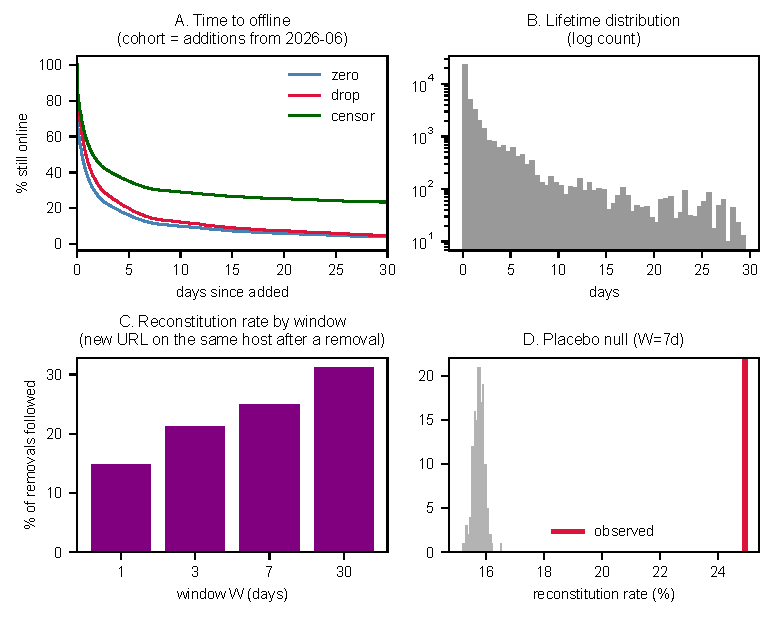
\includegraphics[width=0.58\textwidth]{figures/E7inf_v2.pdf}
\caption{Reconstitution of hosting infrastructure after takedown (E7-inf), in
four views. (a) Time from first sighting to going offline, for the cohort added
from 2026-06. (b) The same lifetimes on a logarithmic count axis.
(c) Reconstitution rate against the observation window. (d) Placebo null at
$W = 7$ days, so the observed rate is read against its null and not against
zero. Every duration is a lower bound.\label{fig2}}
\end{figure}

\begin{figure}[htbp]
\centering
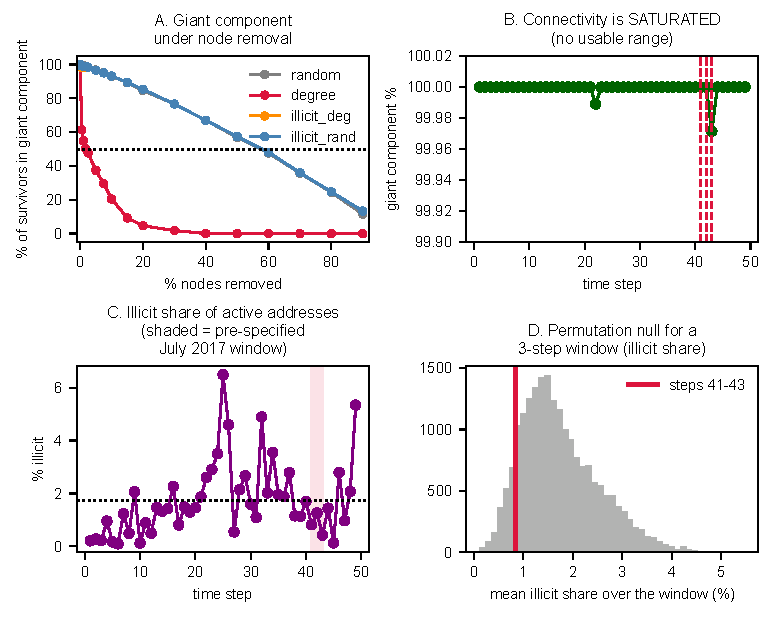
\includegraphics[width=0.58\textwidth]{figures/E6fin_resilience_v2.pdf}
\caption{Dismantling the illicit subgraph (E6-fin), four views on the
Elliptic++ address graph as one aggregate snapshot. (a) Giant component under
node removal. (b) Connectivity across the 49 time steps, saturated and drawn to
record that. (c) Illicit share of active addresses, with the pre-specified
July 2017 window shaded (steps 41--43). (d) Permutation null for that
three-step window.\label{fig3}}
\end{figure}
